\documentclass[10pt,twocolumn,letterpaper]{article}

\usepackage{icb}
\usepackage{times}
\usepackage{epsfig}
\usepackage{graphicx}
\usepackage{amsmath}
\usepackage{amssymb}

\DeclareMathOperator*{\argmin}{arg\,min}

% Include other packages here, before hyperref.

% If you comment hyperref and then uncomment it, you should delete
% egpaper.aux before re-running latex.  (Or just hit 'q' on the first latex
% run, let it finish, and you should be clear).
%\usepackage[pagebackref=true,breaklinks=true,letterpaper=true,colorlinks,bookmarks=false]{hyperref}

%\icbfinalcopy % *** Uncomment this line for the final submission

\def\icbPaperID{****} % *** Enter the IJCB Paper ID here
\def\httilde{\mbox{\tt\raisebox{-.5ex}{\symbol{126}}}}


% Pages are numbered in submission mode, and unnumbered in camera-ready
\ificbfinal\pagestyle{empty}\fi
\begin{document}

%%%%%%%%% TITLE
\title{Effects of using pre-compressed data for compression studies in iris recognition}

\author{First Author\\
Institution1\\
Institution1 address\\
{\tt\small firstauthor@i1.org}
% For a paper whose authors are all at the same institution,
% omit the following lines up until the closing ``}''.
% Additional authors and addresses can be added with ``\and'',
% just like the second author.
% To save space, use either the email address or home page, not both
\and
Second Author\\
Institution2\\
First line of institution2 address\\
{\tt\small secondauthor@i2.org}
}






\maketitle
\thispagestyle{empty}

%%%%%%%%% ABSTRACT
\begin{abstract}
   The ABSTRACT is to be in fully-justified italicized text, at the top
   of the left-hand column, below the author and affiliation
   information. Use the word ``Abstract'' as the title, in 12-point
   Times, boldface type, centered relative to the column, initially
   capitalized. The abstract is to be in 10-point, single-spaced type.
   Leave two blank lines after the Abstract, then begin the main text.
   Look at previous ICB abstracts to get a feel for style and length. 
\end{abstract}

%%%%%%%%% BODY TEXT
\section{Introduction}
Done by Mr. Uhl, including related work?

\section{Test data generation and compression scheme}
\label{section:comprScheme}
We want to investigate the effects of having pre-compressed data falsely assumed as raw data in compression experiments. This means, a pre-compressed image $I_p$ is compressed a second time, hence we denote this process as \emph{double-compression} resulting in an image $I_d$. If a truly uncompressed image $I_u$, which was read directly from the sensor, is compressed, we denote this as \emph{single-compression} resulting in $I_s$. Since experiments are typically carried out on a data base with more than one image, we denote $I_u^{(i)}, I_p^{(i)}, I_s^{(i)}, I_d^{(i)} \in \mathbb{R}^{w \times h}$ as the $i^{th}$ image with width $w$ and height $h$ in the particular data bases. Furthermore, we denote $s(F) \in \mathbb{N}$ with $F \sim{I \in \mathbb{R}^{w \times h}}$ as a function that returns the file size of the file $F$ storing an image $I \in \mathbb{R}^{w \times h} $. Since common compression algorithms employ lossless compression method on the pixel data before writing to a file, $F$ is loosely linked to the contained pixel data $I$. For simplicity, we denote $s(I)$ as the file size of the file $F$ encoding the pixel values of an image $I$. $c_{m}(I, q)$ with $q \in \mathbb{N}$ defines the compression function, which compresses an image $I$ using the quality parameter $q$ with a certain method $m$. In terms of this paper we use the values $m \in \{jpg, jxr, j2k\}$, where 
\begin{itemize}
	\item $jpg$ corresponds to the well-known (ISO/IEC IS 10918-1) DCT-based image compression method \cite{jpg},
	\item $j2k$ corresponds to the wavelet-based image compression standard (ISO/IEC IS 15444-1), which can operate at higher compression ratios \cite{j2k} and
	\item $jxr$ corresponds to a compression standard based on Microsoft’s HD Photo is known to produce higher quality than JPEG, but provides faster conversion than JPEG 2000, as specified in (ISO/IEC IS 29199-2) \cite{jxr}.  
\end{itemize}

%TODO: Consider: Do I have to specify which methods we used (Matlab JxrEncApp) to come up with the images? As it is a standard, this shouldn't be necessary, because everything operates the same anyway?!

For rating the effectiveness of a compression of an image $I$, we define the compression ratio $cr$ between an uncompressed image $I_u$ and a compressed image $I_c$ as 
\begin{equation}
cr(I_u, I_c) = \frac{s(I_u)}{s(I_c)} \quad \text{with} \quad I_c \in \{I_d, I_s\}
\end{equation}

For the later described experiments, images are compressed to meet an arbitrary but fixed target compression ratio $cr_t \in \mathbb{R}$. All three compression methods take one parameter $q \in \mathbb{N}$ only, which controls the image quality but not the file size of the output image. Hence it is not possible to set this parameter in a way to meet a certain target compression ratio $cr_t$. Due to the limited universe of the quality parameters, the target compression ratio $cr_t$ is usually not met exactly, but a parameter optimization can be done, so that $cr_t \approxeq cr^{(i)}$. We propose the following algorithm to compress a data set of uncompressed images $I_u$ with a particular method m to meet a certain compression ratio $cr_t := \gamma$ with $\gamma \in \mathbb{R}$ , e.g. $cr_t := 50$ in a way that the compression ratio of each image is met as close as possible. This process is illustrated in Fig. \ref{fig:comprScheme}.

\begin{figure}[h]
	\begin{center}
		
	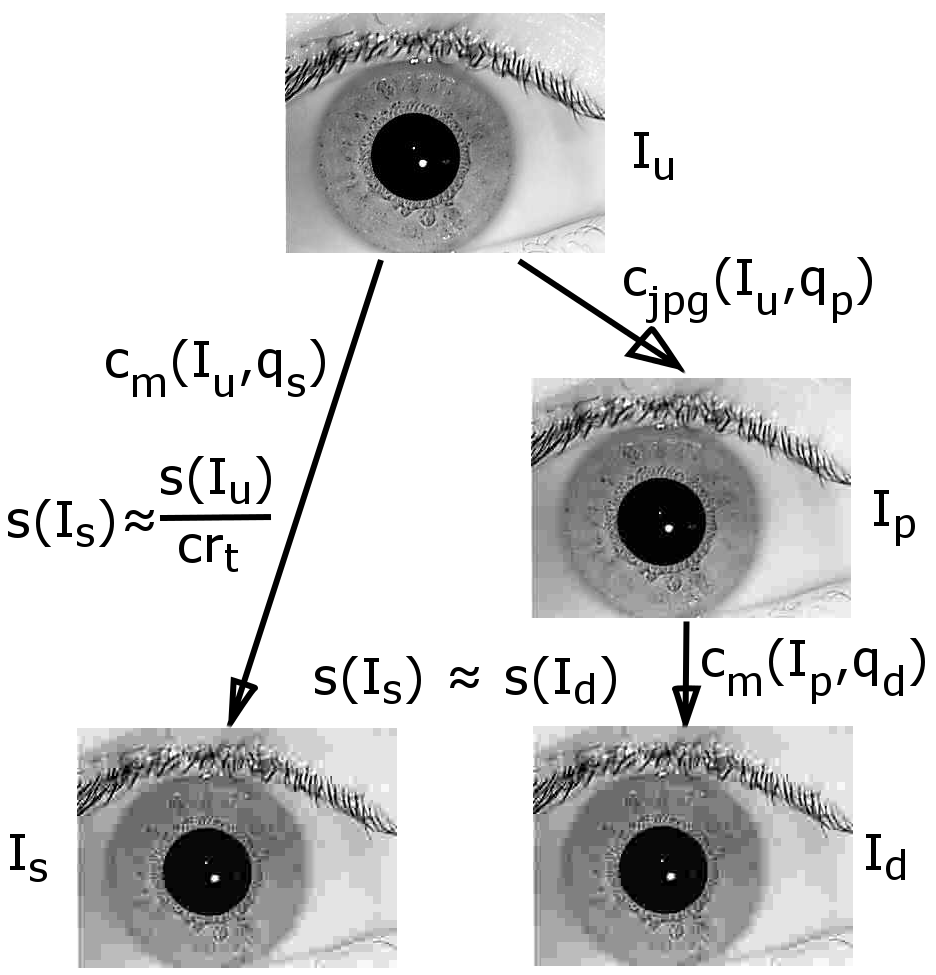
\includegraphics[width=0.7\linewidth]{img/comprScheme}
\end{center}
	\caption{Basic compression principle to obtain two images achieving approximately the same target compression ratio $cr_t$ from an uncompressed image $I_u^{(i)}$ using a particular compression method $m$.One image, $I_s^{(i)}$, is compressed in a single step while the other, $I_d^{(i)}$, uses a pre-compression and a final compression step. Note the pre-compression step is always a $jpg$-compression, while the final compression step uses the same method $m$ as used in the single-compression.}
	\label{fig:comprScheme}
	
\end{figure}

\begin{enumerate}
	\item Compute the single compressed image $I_s^{(i)}$ with method $m$ such that $cr(I_u^{(i)}, I_s^{(i)}) \approx cr_t$. The optimal quality parameter $q_s^{(i)}$ is computed for each image by solving
	\begin{eqnarray}
	\small
	s_t^{(i)} = \frac{s(I_u^{(i)})}{cr_t} \\
		q_s^{(i)} = \underset{q}{argmin}|s(c_m(I_u^{(i)},q)) - s_t^{(i)}|,
	\end{eqnarray} where $s_t^{(i)}$ is the desired file size for matching the target compression ratio $cr_t$ exactly. This is implemented by iteratively searching for the quality parameter $q$ that produces the closest compression ratio $cr(I_u, I_c)$ to the compression ratio $cr_t$. 
	\item The single compressed images $I_s^{(i)}$ with method $m$ are then computed with the found optimal parameters as
	\begin{equation}
	I_s^{(i)} = c_m(I_u^{(i)}, q_s{(i)})
	\end{equation}
	
	\item Compute a pre-compressed image $I_p^{(i)}$, which represents the images in a potentially pre-compressed data base in other experiments. This is done using $jpg$-method \cite{jpg} with an arbitrary but fixed quality parameter $q_p$. Note that images of one data base may have significant variation in terms of file-sizes.
	
	\item Now, find a quality parameter $q_d^{(i)}$ that allows to compress the pre-compressed image $I_p^{(i)}$ a second time, such that the resulting double-compressed image $I_d^{(i)}$ has the same file size as the single compressed image $I_s^{(i)}$, i.e. $s(I_s^{(i)}) \approxeq s(I_d^{(i)})$. Such a quality parameter can be found by 
	\begin{equation}
	\small
		q_d^{(i)} = \underset{q}{argmin}|s(c_m(I_p^{(i)},q)) - s(I_s^{(i)})| \quad \forall s(I_s^{(i)}) \geq s(I_d^{(i)})
	\end{equation}
	
	The condition $s(I_s^{(i)}) \geq s(I_d^{(i)})$ is of special importance to establish fair and defined conditions, since it is very likely that the size cannot be equalized due to the limited universe of the quality parameters of the used compression methods $m$.
	
	\item The double-compressed images $I_p^{(i)}$ are then computed from the pre-compressed images with the found optimal parameters as
	\begin{equation}
		I_d^{(i)} = c_m(I_p^{(i)}, q_d{(i)})
	\end{equation}
	
\end{enumerate}

\section{Experimental setup}
Although there are several iris data sets around, few available in uncompressed format. We use the IITD Iris data base\footnote{IITD Iris Database version 1.0, http://www4.comp.polyu.edu.hk/\textasciitilde csajaykr/IITD/Database\_Iris.htm}. The main reason for this is the availability of a segmentation ground truth created by an expert, which was recently introduced by Rathgeb \etal in \cite{severeCompression}. They also proposes segmentation error results compareable to those we defined in %TODO equations. 
We want to point out that although it is claimed that the data base is in uncompressed BMP format (backed by \cite{severeCompression}), visual evaluation suggests there are slight block artefacts contained, potentially employed by compression. %TODO Can we write it this way? Does this void the complete results?!

We use the scheme introduced in section \ref{section:comprScheme} and compress the data for the following set of target compression ratios:
\begin{equation}
cr_t \in \{5,10,15,20,25,30,35,40,50,60,75\}
\end{equation}
For each of these target compression ratios $cr_t$, the pre-compression step in double-compression mode is carried out with the quality parameters
\begin{equation}
q_p \in \{100, 85, 75, 70\}
\end{equation} 
in order to simulate different levels of pre-compression. Each of these combinations is used to compress with the introduced $jpg$, $j2k$ and $jxr$ methods. This results in a total of 165 data sets with 2240 images each.

\textbf{TODO: Statistics of compression accuracy (mean) and stddev}.

This test data set is used to test six implementations of iris recognition algorithms available in the University of Salzburg Iris Toolbox USIT \cite{rathgeb}.



\section{Evaluation}
 Besides assessing the image quality with fully-referenced metrics, we investigate the behaviour of segmentation error rate and the system's EER in respect to the compression ratio.


\subsection{Full-referenced quality metrics}
Todo Lefteris:
\begin{itemize}
 \item Which quality metrics were in the selection
 \item Which were chosen
 \item Why have you chosen these
 \item Give a very very brief introduction (rather referencing!) of what the quality metrics are about and the most characteristic features
 \item Results and findings of this evaluation
\end{itemize}

\subsection{Segmentation error rates}
TODO TB:
\begin{itemize}
 \item Transform CR's in bpp
 \item Check whether our method is the same as E1 and/or E2 from this paper: \cite{severeCompression}
 \item If not, impl. E1, is E2 also necessary?
 \item Compare referenced to non-referenced
 \item Comparision
 \item Can we probably use their data to draw longer graphs
 \item Results and Findings of this evaluation
\end{itemize}


\subsection{Equal Error rate}
To assess the total impact on the System, the EER is computed
TODO TB

\begin{itemize}
 \item Brief introduction
 \item Results and findings of this evaluation
\end{itemize}


\section{Results}
\subsection{Schnoell-Correlation-method}
TODO: Martin: Introduce your method here and argue why it is better than spearman

\subsection{Correlation of Evaluation methods}
TODO: Martin:
Provide sensible correlation results and analyse


\section{Conclusion}
TODO: Martin Schnöll


{\small
\bibliographystyle{ieee}
\bibliography{egbib}
}

\end{document}
